\documentclass{beamer}
\usepackage{amsmath}
\usepackage{amssymb}
\usepackage{mathrsfs}
\usepackage{amsthm}
\usepackage[utf8]{inputenc}
\usepackage{thmtools,thm-restate}
\usepackage{bm}
\usepackage[italian]{babel}
\usepackage{graphicx}
\usepackage{textpos}
\usepackage{bbm}
\usepackage{caption}
%\usepackage{subcaption}
\usepackage{subfigure}


\usetheme{Madrid}
\setbeamertemplate{blocks}[rounded][shadow=true]
\setbeamertemplate{footline}
{
  \leavevmode%
  \hbox{%
  \begin{beamercolorbox}[wd=.4\paperwidth,ht=2.25ex,dp=1ex,center]{author in head/foot}%
    \usebeamerfont{author in head/foot}\insertshortauthor
  \end{beamercolorbox}%
  \begin{beamercolorbox}[wd=.6\paperwidth,ht=2.25ex,dp=1ex,center]{title in head/foot}%
    \usebeamerfont{title in head/foot}\insertshorttitle\hspace*{3em}
    \insertframenumber{} / \inserttotalframenumber\hspace*{1ex}
  \end{beamercolorbox}}%
  \vskip0pt%
}

\newcommand{\bbR}{\mathbb{R}}
\newcommand{\bbZ}{\mathbb{Z}}
\newcommand{\de}{\partial}
\newcommand*\diff{\mathop{}\!\mathrm{d}}
\newcommand{\OO}{\mathcal{O}}
\newcommand{\AAA}{\mathcal{A}}
\newcommand{\F}{\mathcal{F}}
\newcommand{\Ft}{\widetilde{\F}}
\newcommand{\R}{\mathcal{R}}
\newcommand{\Id}{\mathrm{Id}}
\newcommand{\1}{\mathbbm{1}}
\newcommand{\rmP}{\mathrm{P}}

 
%Information to be included in the title page:
\title{Sample title}
\author[Marco Miani]{Relatore: Stefano Marmi\\
\vspace{5pt}
Studente: Marco Miani
\vspace{10pt}}
\institute{Scuola Normale Superiore}
\date{30 aprile 2019}
 \title[Filtraggio della Matrice di Correlazione] %optional
{Filtraggio della Matrice di Correlazione}

\begin{document}
 
\begin{frame}[plain]
	\maketitle
\end{frame}


\begin{frame}{Introduzione}
Sia $(\Omega,\mathrm{P},\mathcal{F})$ un qualsiasi spazio di probabilità e sia $X:\Omega\mapsto\bbR^n$ una V.A vettoriale su tale spazio.
\[
X=(X_1,\dots,X_n)
\]
\pause
Consideriamo $t$ eventi $\omega_1,\dots,\omega_t$ e prendiamone le immagini tramite $X$ e mettiamole come colonne di una matrice
\[
M = 
\left(
\begin{array}{c}
X_1(\omega_1) \\
\vdots \\
X_n(\omega_1) \\
\end{array}
\left|
\begin{array}{c}
\\
\quad \dots \quad \\
\\
\end{array}
\right|
\begin{array}{c}
X_1(\omega_t) \\
\vdots \\
X_n(\omega_t) \\
\end{array}
\right)
\quad \in \mathfrak{M}(n,t,\mathbb{R})
\]
che chiameremo matrice delle realizzazioni.
\end{frame}

\begin{frame}{Introduzione}
\begin{block}{Covarianza}
$(\Sigma)_{i,j} := \mathrm{Cov}(X_i,X_j) = \mathbb{E}[X_iX_j] = \displaystyle\int_\Omega X_i(\omega)X_j(\omega) \diff \mathrm{P}(\omega)$
\end{block}
\pause
\begin{block}{Covarianza "discreta"}
$\displaystyle (C)_{i,j} := \frac{(MM^T)_{i,j}}{t} = \frac{1}{t}\sum_{s=1}^t M_{i,s}M_{j,s} = \frac{1}{t}\sum_{s=1}^t X_i(\omega_s) X_j(\omega_s)$
\end{block}
\pause
La legge dei grandi numeri ci dice che
\[
\lim_{t \to \infty} \frac{(MM^T)_{i,j}}{t} = (\Sigma)_{i,j}
\]
E quindi per $t$ abbastanza grande si ha $\Sigma \approx C$

\end{frame}

\begin{frame}{Kelly e Markowitz}
L'importanza della matrice $\Sigma$ risulta ancor più evidente dopo aver visto alcuni risultati

\pause
\begin{block}{Criterio di Kelly}
Data una certa scommessa e un certo capitale, ci chiediamo quale sia la percentuale $f^*$ del capitale da investire che massimizza il guadagno.
\[
f^*_{ottimale} = \arg\min \left\{\mathbb{E}[\log(return(f^*))] \,\,|\,0\leq f^*\leq1 \right\}
\]
\end{block}
\pause
\begin{block}{Proiettile di Markowitz}
Dato un mercato, ci chiediamo quale sia il portfolio $W$ di rischio minimo con un dato ritorno $\mu$
\[
W_{ottimale}(\mu) = \arg\min \left\{ W\Sigma W^T \,\,|\,\mu=MW \right\}
\]
\end{block}
\end{frame}


\begin{frame}{Filtraggio}
Se $\Sigma$ è ignota e conosciamo solo $C$? (e.g. corse di cavalli, stock in borsa...)

\pause
\begin{block}{Definizione}
Un filtraggio nella sua forma più generale è un qualsiasi operatore
\[
(filt):\,\mathfrak{M}(n,\bbR) \to \mathfrak{M}(n,\bbR)
\]
Noi considereremo solo filtraggi tra matrici simmetriche definite positive 
\end{block}
Chiameremo:\\
\quad -filtraggio nullo $(filt_{nullo}):=Id_{\mathfrak{M}(n,\bbR)}$.\\
\quad -filtraggio ideale quello tale che $C^{(filt_{ideale})}=\Sigma \qquad \forall C$ realizzazione.

\vspace{15pt}
\pause
Esamineremo 4 tipi di filtraggio:\\
\[
\underbrace{\fbox{SLCA} \qquad\qquad \fbox{ALCA}}_\text{su grafi}
 \qquad\qquad 
\underbrace{\fbox{Rosenow} \qquad\qquad \fbox{Potters}}_\text{spettrali}
\]
\end{frame}

\begin{frame}{Filtraggio con metodi su grafi}
Si costruisce un grafo completo pesato $(N,E,W)$.
\begin{itemize}
\item I nodi $N=\{1,\dots,n\}$ corrispondono alle componenti della V.A. $X$
\item Gli archi $E$ sono tutte le possibili coppie di nodi (grafo completo)
\item Come pesi assegnamo quelli naturali $W(i,j):=C_{i,j}$
\end{itemize}
\vspace{20pt}\pause
Si selezionano gli archi più "significativi" costruendo il Maximum Spanning Tree relativo al grafo.

\vspace{20pt}\pause
Mentre procede l'algoritmo sul grafo, al passo $s$ aggiorniamo la relativa matrice $C^{(s)}$ in modo opportuno.
\end{frame}

\begin{frame}{Filtraggio con metodi su grafi}
\begin{block}{MST - Algoritmo di Kruskal}
All'inizio ci sono $n$ cluster, ciascuno composto da un singolo nodo, e poi si procede iterativamente.\\
\begin{itemize}
\item Si seleziona l'arco di peso maggiore.\\
\item Si uniscono i due cluster di nodi che sono collegati da tale arco.\\
\item Si eliminano gli archi interni ai cluster.
\end{itemize}
Dopo $n-1$ iterazioni si ha solo un cluster e l'algoritmo termina.\\
\end{block}
\begin{picture}(400,80)%
    \put(-10,0){\includegraphics[width=70pt]{kruskal_1.png}}%
    \put(60,65){\color[rgb]{0,0,0}\makebox(0,0)[lb]{\smash{$\curvearrowright$}}}%
    \put(64,0){\includegraphics[width=70pt]{kruskal_2.png}}%
    \put(134,65){\color[rgb]{0,0,0}\makebox(0,0)[lb]{\smash{$\curvearrowright$}}}%
    \put(138,0){\includegraphics[width=70pt]{kruskal_3.png}}%
    \put(208,65){\color[rgb]{0,0,0}\makebox(0,0)[lb]{\smash{$\curvearrowright$}}}%
    \put(212,0){\includegraphics[width=70pt]{kruskal_4.png}}%
    \put(282,65){\color[rgb]{0,0,0}\makebox(0,0)[lb]{\smash{$\curvearrowright$}}}%
    \put(286,0){\includegraphics[width=70pt]{kruskal_5.png}}%
\end{picture}
\end{frame}

\begin{frame}{Filtraggio con metodi su grafi}
\begin{block}{Filtraggio 1 - SLCA (Med)}
Al passo $s$, quando uniamo i cluster H e K nel cluster Q poniamo
\vspace{-5pt}
\[
\displaystyle C^{(s+1)}_{i,j} = \left\{
\begin{array}{ccl}
\displaystyle \frac{|H|\, C^{(s)}_{H,j} + |K|\, C^{(s)}_{K,j}}{|H| + |K|}  & & \text{se } i\in Q \quad j\not\in H\cup K \\
\\
\displaystyle C^{(s)}_{i,j} & & \text{altrimenti}
\end{array}
\right.
\]
\end{block}
\pause
\begin{block}{Filtraggio 2 - ALCA (Max)}
Al passo $s$, quando uniamo i cluster H e K nel cluster Q poniamo
\vspace{-5pt}
\[
\displaystyle C^{(s+1)}_{i,j} = \left\{
\begin{array}{ccl}
\displaystyle \max\{ C^{(s)}_{H,j} , C^{(s)}_{K,j} \}  & & \text{se } i\in Q \quad j\not\in H\cup K \\
\\
\displaystyle C^{(s)}_{i,j} & & \text{altrimenti}
\end{array}
\right.
\]
\end{block}
\pause
Alla fine si pone $C^{(filt)} = C^{(n-1)}$
\end{frame}

\begin{frame}{Filtraggio con metodi spettrali}
Si diagonalizza C tramite matrici ortogonali $C = V^TD\,V$ e si modifica la matrice $D$, operando sugli autovalori più piccoli ($\leq \lambda_{max}$ fissato).
\[
D\rightsquigarrow\tilde{D}
\]
\pause
Si rimoltiplica, ottenendo $\tilde{C} := V^T\tilde{D}\,V$ e si modifica $\tilde{C}$ per assicurarsi che il risultato sia ancora una matrice di correlazione.
\[
\tilde{C}\rightsquigarrow C^{(filt)}
\]

\end{frame}

\begin{frame}{Filtraggio con metodi spettrali}
\vspace{-5pt}
\begin{block}{Filtraggio 3 - Rosenow}
Si sostituiscono gli elementi di D più piccoli di $\lambda_{max}$ con 0
\vspace{-8pt}
\[
\tilde{D}_{i,i} = \left\{
\begin{array}{ccl}
D_{i,i}  & & \text{se } D_{i,i}\geq \lambda_{max} \\
0 & & \text{se } D_{i,i} < \lambda_{max} 
\end{array}
\right.
\]
\vspace{-13pt}

Si forzano gli elementi della diagonale a 1
\vspace{-10pt}
\[
C^{(filt)}_{i,j} = \delta_{i,j} + (1-\delta_{i,j})\tilde{C}_{i,j}
\]
\end{block}
\pause
\vspace{-5pt}
\begin{block}{Filtraggio 4 - Potters}
Si sostituiscono gli elementi di D più piccoli di $\lambda_{max}$ con la loro media
\vspace{-10pt}
\[
\tilde{D}_{i,i} = \left\{
\begin{array}{ccl}
D_{i,i}  & & \text{se } D_{i,i}\geq \lambda_{max} \\
\mathbb{E}[\lambda_j : \lambda_j<\lambda_{max}] & & \text{se } D_{i,i} < \lambda_{max} 
\end{array}
\right.
\]
\vspace{-10pt}

Si pone scalano gli elementi di $\tilde{C}$ con le radici degli elementi diagonali
\vspace{-10pt}
\[
C^{(filt)}_{i,j} = \frac{\tilde{C}_{i,j}}{\sqrt{\tilde{C}_{i,i} \, \tilde{C}_{j,j}}}
\]
\end{block}
\end{frame}



\begin{frame}{Stima bontà del filtraggio}
\begin{itemize}
\item Fissiamo una V.A. vettoriale con matrice di covarianza $\Sigma\in\mathfrak{M}(n,\bbR)$ simmetrica definita positiva
\pause
\item Costruiamo tante ($\sim 1000$) sue realizzazioni indipendenti $M_1,\dots,M_{1000}\in\mathfrak{M}(n,t,\bbR)$ 
\pause
\item Calcoliamo le matrici di covarianza $C_1,\dots,C_{1000}\in\mathfrak{M}(n,\bbR)$ associate alle rispettive realizzazioni
\pause
\item Scegliamo un filtraggio e applichiamolo, ottenendo $C^{(filt)}_1,\dots,C^{(filt)}_{1000}$
\end{itemize}
\pause
\hspace{60pt} \begin{tabular}{clccc}
			&				&\onslide<6,7>{$C_1$}					&\onslide<7>{$\rightarrow$}	&\onslide<7>{$C^{(filt)}_1$}\\
			&\onslide<6,7>{$\nearrow$}	&\onslide<6,7>{$\vdots$}	&				&\onslide<7>{$\vdots$}\\
$\Sigma$	&\onslide<6,7>{$\rightarrow$}	&\onslide<6,7>{$C_i$}	&\onslide<7>{$\rightarrow$}	&\onslide<7>{$C^{(filt)}_1$}\\
			&\onslide<6,7>{$\searrow$}	&\onslide<6,7>{$\vdots$}	&				&\onslide<7>{$\vdots$}\\
			&				&\onslide<6,7>{$C_{1000}$}				&\onslide<7>{$\rightarrow$}	&\onslide<7>{$C^{(filt)}_1$}
\end{tabular}
\end{frame}

\begin{frame}{Stima bontà del filtraggio}
Fissiamo una distanza tra matrici $d:\mathfrak{M}(n,\bbR)\times\mathfrak{M}(n,\bbR) \to \bbR^+$.
\pause
\vspace{10pt}

Per capire quanto un $(filt) \approx (filt_{ideale})$ possiamo misurare:
\vspace{5pt}
\begin{enumerate}
\item Quanto $C^{(filt)}$ si avvicina a $\Sigma$?\\
	\vspace{2pt}
	\quad $\displaystyle\langle d(\Sigma,C^{(filt)}) \rangle \onslide<3>{:= \frac{1}{1000}\sum_{i=1}^{1000} d(\Sigma,C^{(filt)}_i)}$
	\vspace{4pt}
\item Quanta informazione di $C$ viene persa/trattenuta in $C^{(filt)}$?\\
	\vspace{2pt}
	\quad $\displaystyle\langle d(C,C^{(filt)}) \rangle \onslide<3>{:= \frac{1}{1000}\sum_{i=1}^{1000} d(C,C^{(filt)}_i)}$
	\vspace{4pt}
\item Quanto è stabile il filtraggio?\\
	\quad $\displaystyle\langle d(C^{(filt)},C^{(filt)}) \rangle \onslide<3>{:= \frac{1}{499500}\sum_{\substack{i,j=1 \\ i\neq j}}^{1000} d(C^{(filt)}_i,C^{(filt)}_j)}$
\end{enumerate}
\end{frame}

\begin{frame}{Stima bontà del filtraggio}
\begin{picture}(200,200)%
    \put(98,98){\color[rgb]{0,0,0}\makebox(0,0)[lb]{\smash{$\bullet$}}}%
    \put(103,103){\color[rgb]{0,0,0}\makebox(0,0)[lb]{\smash{$\Sigma$}}}%
    \pause
    \put(70,200){\color[rgb]{0,0,0}\makebox(0,0)[lb]{\smash{$\bullet C_1$}}}%
    \pause
    \put(110,175){\color[rgb]{0,0,0}\makebox(0,0)[lb]{\smash{$\bullet C_2$}}}%
    \put(175,175){\color[rgb]{0,0,0}\makebox(0,0)[lb]{\smash{$\bullet C_3$}}}%
    \put(210,120){\color[rgb]{0,0,0}\makebox(0,0)[lb]{\smash{$\bullet C_4$}}}%
    \put(180,30){\color[rgb]{0,0,0}\makebox(0,0)[lb]{\smash{$\bullet C_i$}}}%
    \put(70,15){\color[rgb]{0,0,0}\makebox(0,0)[lb]{\smash{$\bullet C_{1000}$}}}%
    \pause
    \put(0,0){\includegraphics[width=200pt]{cerchi_est.jpg}}%
    \put(98,98){\color[rgb]{0,0,0}\makebox(0,0)[lb]{\smash{$\bullet$}}}%
    \put(103,103){\color[rgb]{0,0,0}\makebox(0,0)[lb]{\smash{$\Sigma$}}}%
    \put(70,200){\color[rgb]{0,0,0}\makebox(0,0)[lb]{\smash{$\bullet C_1$}}}%
    \put(110,175){\color[rgb]{0,0,0}\makebox(0,0)[lb]{\smash{$\bullet C_2$}}}%
    \put(175,175){\color[rgb]{0,0,0}\makebox(0,0)[lb]{\smash{$\bullet C_3$}}}%
    \put(210,120){\color[rgb]{0,0,0}\makebox(0,0)[lb]{\smash{$\bullet C_4$}}}%
    \put(180,30){\color[rgb]{0,0,0}\makebox(0,0)[lb]{\smash{$\bullet C_i$}}}%
    \put(70,15){\color[rgb]{0,0,0}\makebox(0,0)[lb]{\smash{$\bullet C_{1000}$}}}%
    \pause
    \put(60,140){\color[rgb]{0,0,0}\makebox(0,0)[lb]{\smash{$\bullet C_1^{(filt)}$}}}%
    \pause
    \put(95,130){\color[rgb]{0,0,0}\makebox(0,0)[lb]{\smash{$\bullet C_2^{(filt)}$}}}%
    \put(145,135){\color[rgb]{0,0,0}\makebox(0,0)[lb]{\smash{$\bullet C_3^{(filt)}$}}}%
    \put(145,100){\color[rgb]{0,0,0}\makebox(0,0)[lb]{\smash{$\bullet C_4^{(filt)}$}}}%
    \put(125,50){\color[rgb]{0,0,0}\makebox(0,0)[lb]{\smash{$\bullet C_i^{(filt)}$}}}%
    \put(70,65){\color[rgb]{0,0,0}\makebox(0,0)[lb]{\smash{$\bullet C_{1000}^{(filt)}$}}}%
    \pause
    \put(0,0){\includegraphics[width=200pt]{cerchi.jpg}}%
    \put(98,98){\color[rgb]{0,0,0}\makebox(0,0)[lb]{\smash{$\bullet$}}}%
    \put(103,103){\color[rgb]{0,0,0}\makebox(0,0)[lb]{\smash{$\Sigma$}}}%
    \put(70,200){\color[rgb]{0,0,0}\makebox(0,0)[lb]{\smash{$\bullet C_1$}}}%
    \put(110,175){\color[rgb]{0,0,0}\makebox(0,0)[lb]{\smash{$\bullet C_2$}}}%
    \put(175,175){\color[rgb]{0,0,0}\makebox(0,0)[lb]{\smash{$\bullet C_3$}}}%
    \put(210,120){\color[rgb]{0,0,0}\makebox(0,0)[lb]{\smash{$\bullet C_4$}}}%
    \put(180,30){\color[rgb]{0,0,0}\makebox(0,0)[lb]{\smash{$\bullet C_i$}}}%
    \put(70,15){\color[rgb]{0,0,0}\makebox(0,0)[lb]{\smash{$\bullet C_{1000}$}}}%
    \put(60,140){\color[rgb]{0,0,0}\makebox(0,0)[lb]{\smash{$\bullet C_1^{(filt)}$}}}%
    \put(95,130){\color[rgb]{0,0,0}\makebox(0,0)[lb]{\smash{$\bullet C_2^{(filt)}$}}}%
    \put(145,135){\color[rgb]{0,0,0}\makebox(0,0)[lb]{\smash{$\bullet C_3^{(filt)}$}}}%
    \put(145,100){\color[rgb]{0,0,0}\makebox(0,0)[lb]{\smash{$\bullet C_4^{(filt)}$}}}%
    \put(125,50){\color[rgb]{0,0,0}\makebox(0,0)[lb]{\smash{$\bullet C_i^{(filt)}$}}}%
    \put(70,65){\color[rgb]{0,0,0}\makebox(0,0)[lb]{\smash{$\bullet C_{1000}^{(filt)}$}}}%
    
    \pause
    \put(250,170){\includegraphics[width=40pt]{cerchietti_1.png}}%
    \put(250,155){\color[rgb]{0,0,0}\makebox(0,0)[lb]{\smash{$\langle d(\Sigma,C^{(filt)}) \rangle$}}}%
    \pause
    \put(250,90){\includegraphics[width=40pt]{cerchietti_2.png}}%
    \put(250,75){\color[rgb]{0,0,0}\makebox(0,0)[lb]{\smash{$\langle d(C,C^{(filt)}) \rangle$}}}%
    \pause
    \put(250,10){\includegraphics[width=40pt]{cerchietti_3.png}}%
    \put(250,-5){\color[rgb]{0,0,0}\makebox(0,0)[lb]{\smash{$\langle d(C^{(filt)},C^{(filt)}) \rangle$}}}%
\end{picture}
\end{frame}

\begin{frame}{Stima bontà del filtraggio}
\begin{picture}(1,1)%
    \onslide<2>{\put(200,-75){\includegraphics[width=130pt]{Plot_base_1.png}}}%
    \onslide<3>{\put(200,-75){\includegraphics[width=130pt]{Plot_base_2.png}}}%
\end{picture}
Se la matrice $\Sigma$ ci è ignota:
\vspace{20pt}
\begin{enumerate}
\item $\langle d(\Sigma,C^{(filt)}) \rangle$ {\color{red} NON calcolabile}\\
\vspace{10pt}
\item $\langle d(C,C^{(filt)}) \rangle$ {\color{green} calcolabile}\\
\vspace{5pt}
\onslide<2,3>{\begin{columns}
\begin{column}{0.1 \textwidth}
\includegraphics[width=40pt]{cerchietti_2.png}
\end{column}
\begin{column}{0.8 \textwidth}
\[
\underbrace{0 = \langle d(C,C)\rangle}_\text{filtraggio nullo}
\leq \langle d(C,C^{(filt)})\rangle \leq 
\underbrace{\langle d(C,\Sigma)\rangle = \text{ ?}}_\text{filtraggio perfetto}
\]
\end{column}
\end{columns}}
\vspace{10pt}
\item $\langle d(C^{(filt)},C^{(filt)}) \rangle$ {\color{green} calcolabile}\\
\vspace{5pt}
\onslide<3>{\begin{columns}
\begin{column}{0.1 \textwidth}
\includegraphics[width=40pt]{cerchietti_3.png}
\end{column}
\begin{column}{0.8 \textwidth}
\[
\underbrace{0 = \langle d(\Sigma,\Sigma)\rangle}_\text{filtraggio perfetto} 
\leq \langle d(C_i^{(filt)},C_j^{(filt)})\rangle \leq
\underbrace{\langle d(C_i,C_j)\rangle = \text{ ?}}_\text{filtraggio nullo}
\]
\end{column}
\end{columns}}
\end{enumerate}
\end{frame}



\begin{frame}{Distanza di Kullback-Leibler}
\begin{block}{Definizione}
Date due densità di probabilità $\mathrm{P}$ e $\mathrm{Q}$ si definisce:
\[
K(\mathrm{P},\mathrm{Q}):=
\mathbb{E}\left[\ln{\left(\frac{\mathrm{P}}{\mathrm{Q}}\right)}\right] =
\int \ln{\left(\frac{\mathrm{P}(x)}{\mathrm{Q}(x)}\right)} \diff\mathrm{P}(x)
\]
la distanza di Kullback-Leibler.
\end{block}
\pause
Proprietà:
\begin{itemize}
\item $K(\mathrm{P},\mathrm{P})=0$
\item $K(\mathrm{P},\mathrm{Q})\geq 0$\\
\qquad $-K(\mathrm{P},\mathrm{Q}) = \int \log(\frac{\mathrm{Q}}{\mathrm{P}})\mathrm{P}\diff x
 \leq log(\int\frac{\mathrm{Q}}{\mathrm{P}}\mathrm{P}\diff x) = \log(1) = 0$
\item \textbf{Non} è simmetrica\\
\qquad $K_{sim}(\mathrm{P},\mathrm{Q}) := K(\mathrm{P},\mathrm{Q}) + K(\mathrm{Q},\mathrm{P}) 
 = \int\log(\frac{\mathrm{P}}{\mathrm{Q}})(\mathrm{P}-\mathrm{Q})\diff x$
\item \textbf{Non} soddisfa la disuguaglianza triangolare
\end{itemize}
\end{frame}

\begin{frame}{Distanza di Kullback-Leibler}
\vspace{-5pt}
\begin{block}{Definizione}
Date due densità di probabilità $\mathrm{P}$ e $\mathrm{Q}$ si definisce:
\[
K(\mathrm{P},\mathrm{Q}):=
\mathbb{E}\left[\ln{\left(\frac{\mathrm{P}}{\mathrm{Q}}\right)}\right] =
\int \ln{\left(\frac{\mathrm{P}(x)}{\mathrm{Q}(x)}\right)} \diff\mathrm{P}(x)
\]
la distanza di Kullback-Leibler.
\end{block}
\vspace{10pt}

Nata originariamente per definire l'\textbf{informazione mutuale} tra Variabili Aleatorie $X$ e $Y$ come
\[
\mathrm{I}(X,Y) := K(\mathbb{P}(X,Y),\mathbb{P}(X)\mathbb{P}(Y))
\]
\vspace{-15pt}
\[
\qquad\qquad\qquad \,=\int \ln{\left(\frac{\mathbb{P}(X,Y)}{\mathbb{P}(X)\mathbb{P}(Y)}\right)} \diff\mathbb{P}(X,Y)
\]
\end{frame}

\begin{frame}{Distanza di Kullback-Leibler}
Consideriamo due variabili aleatorie gaussiane di media nulla e varianza $\Sigma_i$
\[
X_1 \sim \text{N}(0,\Sigma_1) \qquad X_2 \sim \text{N}(0,\Sigma_2)
\]
e le relative densità di probabilità associate
\[
\mathrm{P}_i(x) = \frac{1}{\sqrt{(2\pi)^n\det{(\Sigma_i)}}} e^{-\frac{1}{2}x^T\Sigma_i^{-1}x }
\]
\vspace{10pt}
\pause

Possiamo quindi definire una distanza tra matrici
\begin{block}{Definizione}
Date due matrici simmetriche definite positive $\Sigma_1$ e $\Sigma_2$ si definisce:
\[
K(\Sigma_1,\Sigma_2) := K(\mathrm{P}_1,\mathrm{P}_2)
\]
la distanza di Kullback-Leibler tra matrici.
\end{block}
\end{frame}

\begin{frame}{Distanza di Kullback-Leibler}
\vspace{-15pt}
\begin{align*}
\hspace{-5pt} K(\Sigma_1,\Sigma_2) 
 & = \int \ln{\left(\frac{\mathrm{P}_1(x)}{\mathrm{P}_2(x)}\right)} \diff\mathrm{P}_1(x) \\
 \onslide<3>{ 
 & = \int
 		\ln\left(\sqrt{\frac{\det(\Sigma_2)}{\det(\Sigma_1)}}  e^{-\frac{1}{2}(x^T\Sigma_1^{-1}x - x^T\Sigma_2^{-1}x)}  \right)
 		\diff \rmP_1(x)\\
 & = \int
 		\ln\left(\sqrt{\frac{\det(\Sigma_2)}{\det(\Sigma_1)}}\right) 
 	 \diff \rmP_1(x)
 	 -
 	 \frac{1}{2}\int
 	 	(x^T\Sigma_1^{-1}x - x^T\Sigma_2^{-1}x)
	 \diff \rmP_1(x)\\
 & = \frac{1}{2}\left( 
 		\ln\left(\frac{\det(\Sigma_2)}{\det(\Sigma_1)}\right)
 		+
 		\int x^T\Sigma_2^{-1}x \diff \rmP_1(x)
 		-
 		\int x^T\Sigma_1^{-1}x \diff \rmP_1(x)
 	 \right)\\
 }
 \onslide<2,3>{
 & = \frac{1}{2}\left( 
 		\ln\left(\frac{\det(\Sigma_2)}{\det(\Sigma_1)}\right)
 		+
 		\text{TR}(\Sigma_2^{-1}\Sigma_1)
 		-
 		n
 	 \right)
 }
\end{align*}
\onslide<3>{calcolabile esplicitamente in funzione delle sole matrici $\Sigma_1$ e $\Sigma_2$}
\end{frame}

\begin{frame}{Distanza di Kullback-Leibler}
Delle $C$ così costruite seguono la distribuzione di Wishart
\[
C\sim W_n(\Sigma,t)
\]
\pause
con densità
\[
f(C) = \frac{1}{ \Gamma_n(\frac{t}{2}) \left(\sqrt{2^n\det(\Sigma)}\right)^t } 
(\det(C))^{\frac{t-n-1}{2}}
e^{-\frac{1}{2}\text{TR}(\Sigma^{-1}C)}
\]
dove $\displaystyle
\Gamma_n\left(\frac{t}{2}\right) = 
\pi^{\frac{n(n-1)}{4}}
\prod_{j=0}^{n-1} \Gamma\left(\frac{t-j}{2}\right)$ è la Multivariate Gamma Function.
\vspace{20pt}

\end{frame}

\begin{frame}{Distanza di Kullback-Leibler}
Grazie a questa possiamo calcolare
\[
\mathbb{E}_W[K(\Sigma,C)]
\onslide<2,3>{
	=\frac{1}{2}\left(
	n\ln\left(\frac{2}{t}\right) + 
	\!\sum_{p=t-n+1}^t \left(\frac{\Gamma'(p/2)}{\Gamma(p/2)}\right)\, +
	\,\frac{n(n+1)}{t-n-1}
	\right)
	}
\]
\[
\mathbb{E}_W[K(C,\Sigma)]
\onslide<2,3>{
	=\frac{1}{2}\left(
	n\ln\left(\frac{t}{2}\right) - 
	\!\sum_{p=t-n+1}^t \left(\frac{\Gamma'(p/2)}{\Gamma(p/2)}\right)
	\right)
	}
\]
\[
\mathbb{E}_{W\otimes W}[K(C,C)]
	\onslide<2,3>{
	=\frac{1}{2}\frac{n(n-1)}{t-n-1}
	}
\]
\vspace{10pt}

\onslide<3>{che \textbf{NON} dipendono da $\Sigma$}
\end{frame}



\begin{frame}{Applicazione}

\begin{itemize}
\item $\langle d(C,C^{(filt)}) \rangle$\\
\vspace{3pt}
\begin{columns}
\begin{column}{0.1 \textwidth}
\includegraphics[width=40pt]{cerchietti_2.png}
\end{column}
\begin{column}{0.8 \textwidth}
Quanta informazione di $C$ viene persa/trattenuta in $C^{(filt)}$?
\end{column}
\end{columns}
\[
\underbrace{0 = \langle K(C,C)\rangle}_\text{filtraggio nullo}
\leq \langle K(C,C^{(filt)})\rangle \leq 
\underbrace{\langle K(C,\Sigma)\rangle \approx \mathbb{E}_W[K(C,\Sigma)]}_\text{filtraggio perfetto}
\]
\pause
\vspace{15pt}
\item $\langle d(C^{(filt)},C^{(filt)}) \rangle$\\
\vspace{3pt}
\begin{columns}
\begin{column}{0.1 \textwidth}
\includegraphics[width=40pt]{cerchietti_3.png}
\end{column}
\begin{column}{0.8 \textwidth}
Quanto è stabile il filtraggio?
\end{column}
\end{columns}
\[
\underbrace{0 = \langle K(\Sigma,\Sigma)\rangle}_\text{filtraggio perfetto} 
\leq \langle K(C_i^{(filt)},C_j^{(filt)})\rangle \leq
\underbrace{\langle K(C_i,C_j)\rangle \approx \mathbb{E}_{W\otimes W}[K(C,C)]}_\text{filtraggio nullo}
\]
\end{itemize}
\end{frame}

%\begin{frame}{Applicazione}
%\includegraphics[width=\linewidth]{Plot_base_2.png}
%\end{frame}



\begin{frame}{Applicazione - Test Teorici}
\begin{itemize}
\item Fissiamo $n$ e $t$
\pause
\item Generiamo una $\Sigma$ casuale $\in\mathfrak{M}(n,n,\bbR)$
\pause
\item Costruiamo \textbf{tante} sue realizzazioni indipendenti $M_i\in\mathfrak{M}(n,t,\bbR)$ 
\pause
\item Per ciascuna realizzazione $M_i$ calcoliamo la matrice di covarianza $C_i$
\pause
\item Applichiamo i filtraggi 
\[C_i \rightsquigarrow \left[C^{(filt_{Max})}_i,C^{(filt_{Med})}_i,C^{(filt_{Potter})}_i,C^{(filt_{Rosenow})}_i\right]\]
\pause
\item Calcoliamo le medie delle distanze e plottiamo i 4 punti
\end{itemize}
\[
\left(\, \langle K(C,C^{(filt_{Max})})\rangle , \langle K(C^{(filt_{Max})},C^{(filt_{Max})})\rangle \,\right) \quad\in\bbR^2
\]
\[
\left(\, \langle K(C,C^{(filt_{Med})})\rangle , \langle K(C^{(filt_{Med})},C^{(filt_{Med})})\rangle \,\right) \quad\in\bbR^2
\]
\[
\left(\, \langle K(C,C^{(filt_{Potter})})\rangle , \langle K(C^{(filt_{Potter})},C^{(filt_{Potter})})\rangle \,\right) \quad\in\bbR^2
\]
\[
\left(\, \langle K(C,C^{(filt_{Rosenow})})\rangle , \langle K(C^{(filt_{Rosenow})},C^{(filt_{Rosenow})})\rangle \,\right) \quad\in\bbR^2
\]
\end{frame}

\begin{frame}{Applicazione - Test Teorici}
\centering\includegraphics[width=0.9\linewidth]{Plot_n5_T15_it100_simul1.png}
\end{frame}

\begin{frame}{Applicazione - Test Teorici}
\centering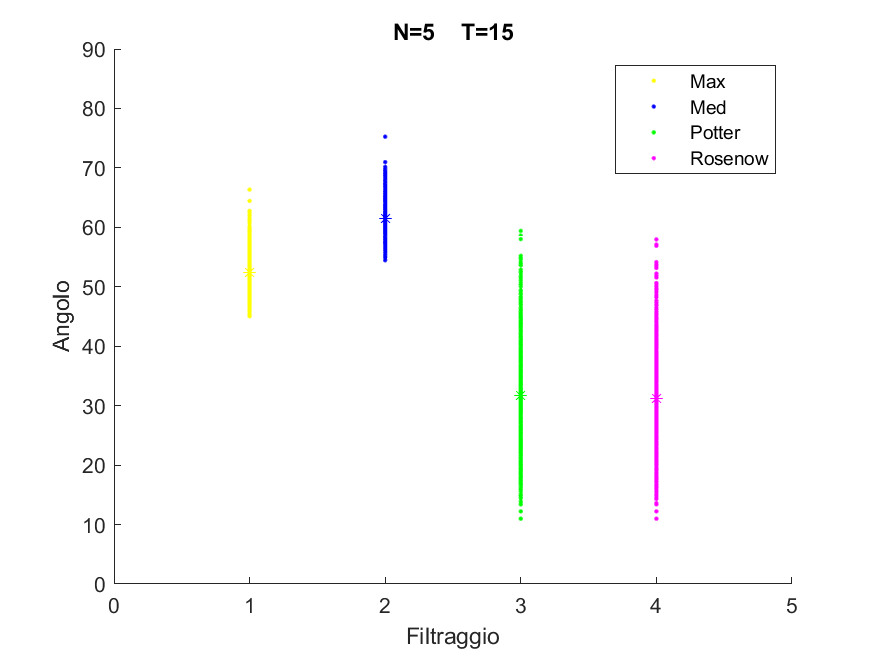
\includegraphics[width=0.9\linewidth]{plot/teorici/Plot_n5_T15_it100_simul1000.png}
\end{frame}

\begin{frame}{Applicazione - Test Teorici (n=4)}
\begin{columns}
\begin{column}{0.5\linewidth}
\includegraphics[width=\linewidth]{plot/teorici/Plot_n4_T6_it100_simul1000.png}
\end{column}
\begin{column}{0.5\linewidth}
\includegraphics[width=\linewidth]{plot/teorici/Plot_n4_T8_it100_simul1000.png}
\end{column}
\end{columns}

\begin{columns}
\begin{column}{0.33\linewidth}
\includegraphics[width=\linewidth]{plot/teorici/Plot_n4_T11_it100_simul1000.png}
\end{column}
\begin{column}{0.33\linewidth}
\includegraphics[width=\linewidth]{plot/teorici/Plot_n4_T14_it100_simul1000.png}
\end{column}
\begin{column}{0.33\linewidth}
\includegraphics[width=\linewidth]{plot/teorici/Plot_n4_T24_it100_simul1000.png}
\end{column}
\end{columns}
\end{frame}

\begin{frame}{Applicazione - Test Teorici (n=10)}
\begin{columns}
\begin{column}{0.5\linewidth}
\includegraphics[width=\linewidth]{plot/teorici/Plot_n10_T14_it100_simul1000.png}
\end{column}
\begin{column}{0.5\linewidth}
\includegraphics[width=\linewidth]{plot/teorici/Plot_n10_T17_it100_simul1000.png}
\end{column}
\end{columns}

\begin{columns}
\begin{column}{0.33\linewidth}
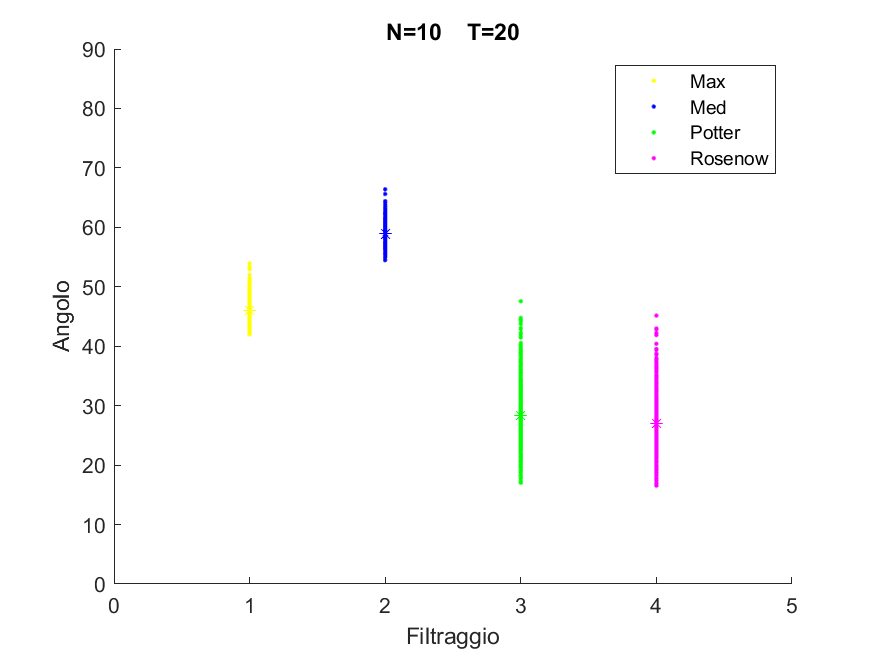
\includegraphics[width=\linewidth]{plot/teorici/Plot_n10_T20_it100_simul1000.png}
\end{column}
\begin{column}{0.33\linewidth}
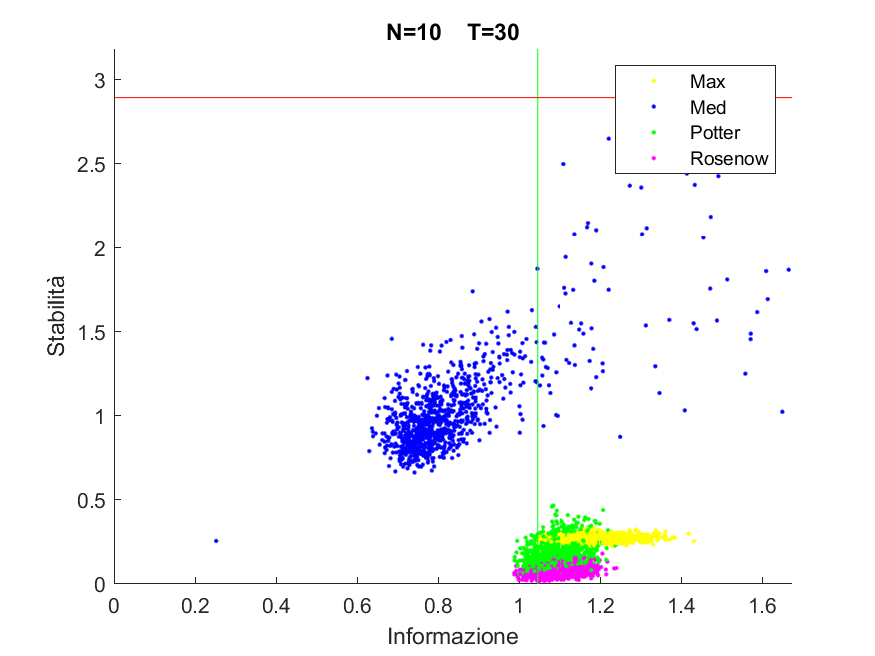
\includegraphics[width=\linewidth]{plot/teorici/Plot_n10_T30_it100_simul1000.png}
\end{column}
\begin{column}{0.33\linewidth}
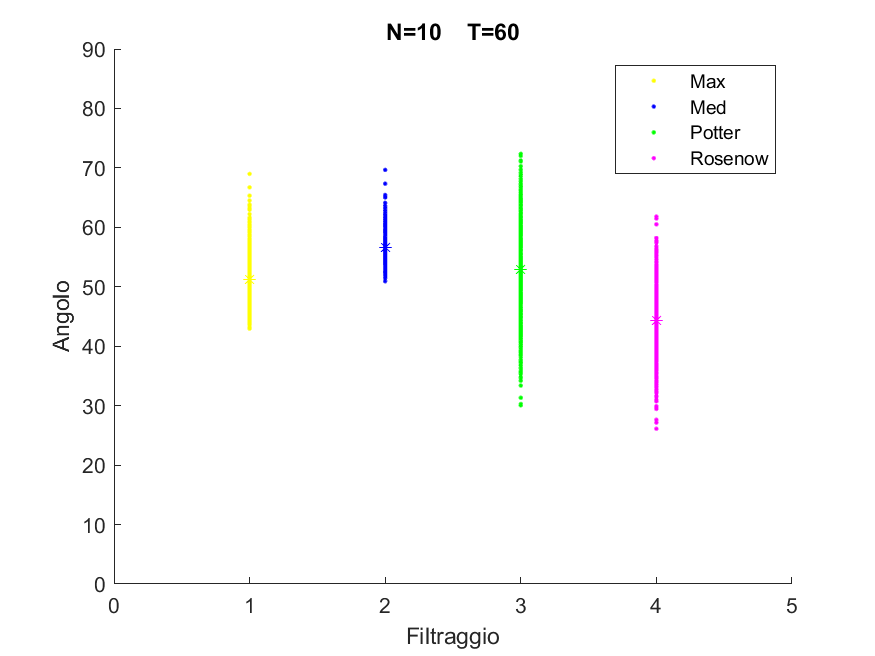
\includegraphics[width=\linewidth]{plot/teorici/Plot_n10_T60_it100_simul1000.png}
\end{column}
\end{columns}
\end{frame}












\begin{frame}{Applicazione - Test Pratici}
\vspace{-140pt}
\begin{picture}(1,1)%
\onslide<2>{\put(-48,-225){\includegraphics[width=1.25\linewidth]{Plottone_giorn.png}}}%
\end{picture}\\
I dati da cui sono partito sono i prezzi in chiusura giornalieri di 7227 stock.\\
Di questi ho selezionati i 2122 che avevano dati per almeno 20 anni
\end{frame}

\begin{frame}{Applicazione - Test Pratici}
Dai prezzi giornalieri sono passato alle medie settimanali e da queste sono passato agli incrementi percentuali tra una settimana e la succssiva.
\begin{columns}
\begin{column}{0.5\linewidth}
\vspace{-30pt}
\[ incr(i)=\frac{prezzo(i)-prezzo(i-1)}{|prezzo(i)|} \]
\end{column}
\pause
\begin{column}{0.6\linewidth}
\centering\includegraphics[width=\linewidth]{Plottone_incr.png}
\end{column}
\end{columns}
\end{frame}

\begin{frame}{Applicazione - Test Pratici}
\begin{itemize}
\item Fissiamo $n$ e $t$
\pause
\item Scegliamo $n$ stock quotati nella borsa di New York
\pause
\item Prendiamo i dati relativi relativi a \textbf{tanti} intervalli di tempo lunghi $t$ disgiunti (=realizzazioni indipendenti $M_i\in\mathfrak{M}(n,t,\bbR)$ )
\pause
\item Per ciascuna realizzazione $M_i$ calcoliamo la matrice di covarianza $C_i$
\pause
\item Applichiamo i filtraggi 
\[C_i \rightsquigarrow \left[C^{(filt_{Max})}_i,C^{(filt_{Med})}_i,C^{(filt_{Potter})}_i,C^{(filt_{Rosenow})}_i\right]\]
\pause
\item Calcoliamo le medie delle distanze e plottiamo i 4 punti
\end{itemize}
\[
\left(\, \langle K(C,C^{(filt_{Max})})\rangle , \langle K(C^{(filt_{Max})},C^{(filt_{Max})})\rangle \,\right) \quad\in\bbR^2
\]
\[
\left(\, \langle K(C,C^{(filt_{Med})})\rangle , \langle K(C^{(filt_{Med})},C^{(filt_{Med})})\rangle \,\right) \quad\in\bbR^2
\]
\[
\left(\, \langle K(C,C^{(filt_{Potter})})\rangle , \langle K(C^{(filt_{Potter})},C^{(filt_{Potter})})\rangle \,\right) \quad\in\bbR^2
\]
\[
\left(\, \langle K(C,C^{(filt_{Rosenow})})\rangle , \langle K(C^{(filt_{Rosenow})},C^{(filt_{Rosenow})})\rangle \,\right) \quad\in\bbR^2
\]
\end{frame}

\begin{frame}{Applicazione - Test Pratici}
\centering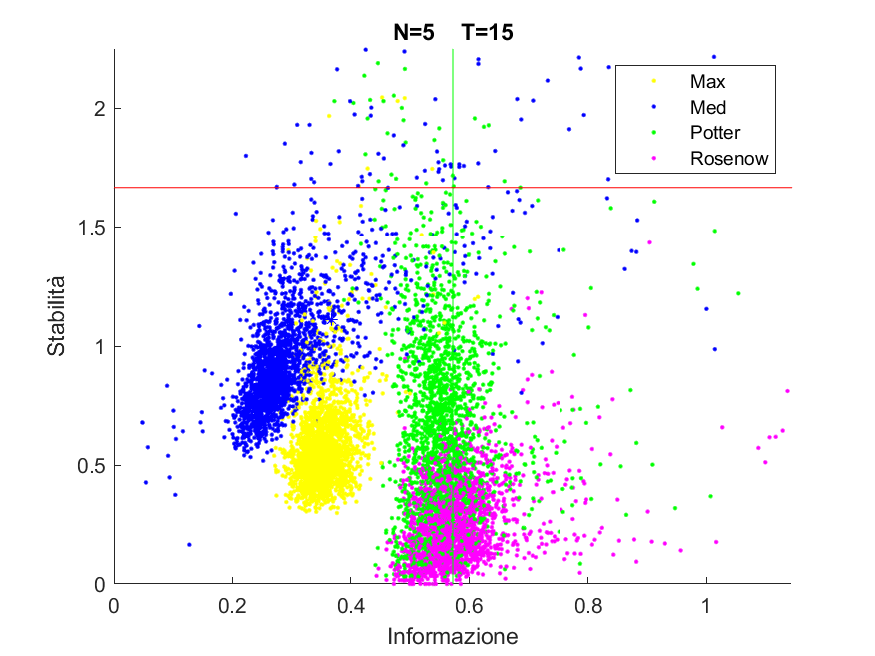
\includegraphics[width=0.9\linewidth]{plot/pratici/Plot_n5_T15.png}
\end{frame}

\begin{frame}{Applicazione - Test Pratici (n=4)}
\begin{columns}
\begin{column}{0.5\linewidth}
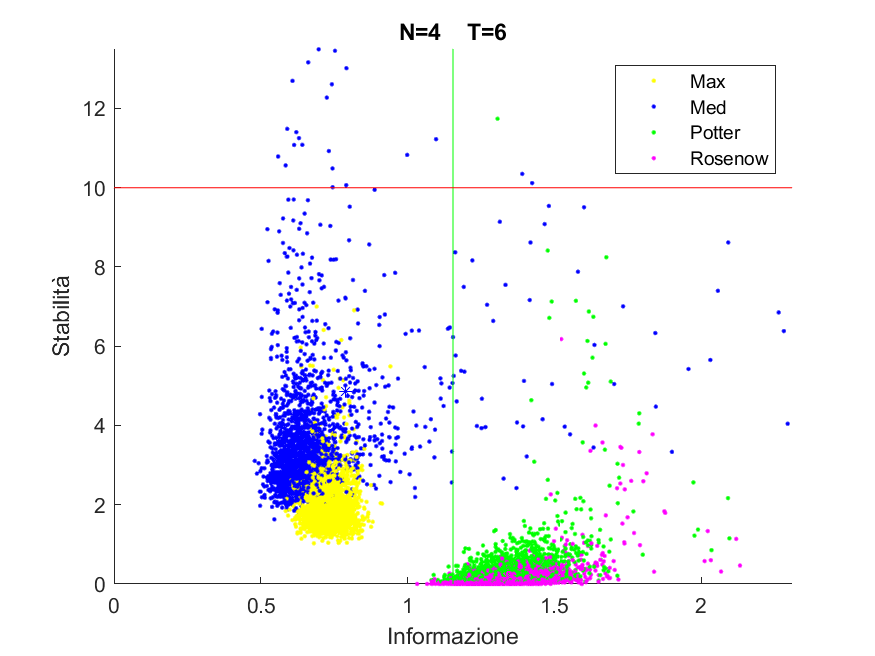
\includegraphics[width=\linewidth]{plot/pratici/Plot_n4_T6.png}
\end{column}
\begin{column}{0.5\linewidth}
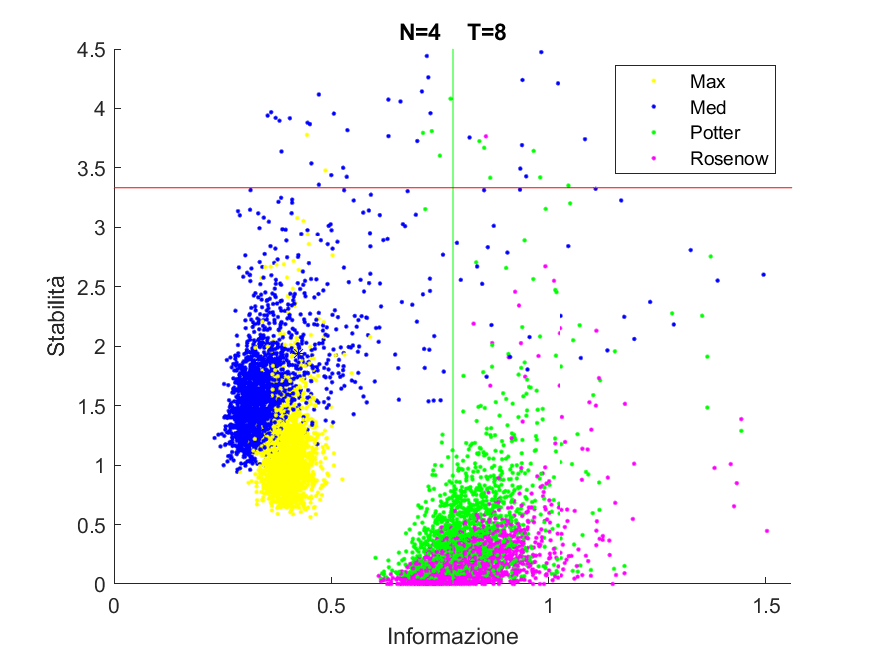
\includegraphics[width=\linewidth]{plot/pratici/Plot_n4_T8.png}
\end{column}
\end{columns}

\begin{columns}
\begin{column}{0.33\linewidth}
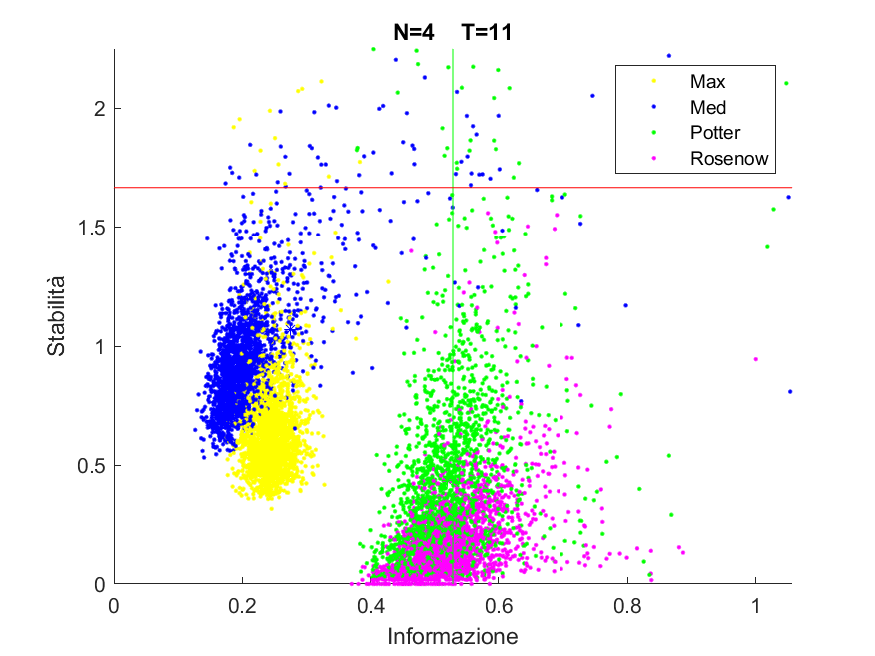
\includegraphics[width=\linewidth]{plot/pratici/Plot_n4_T11.png}
\end{column}
\begin{column}{0.33\linewidth}
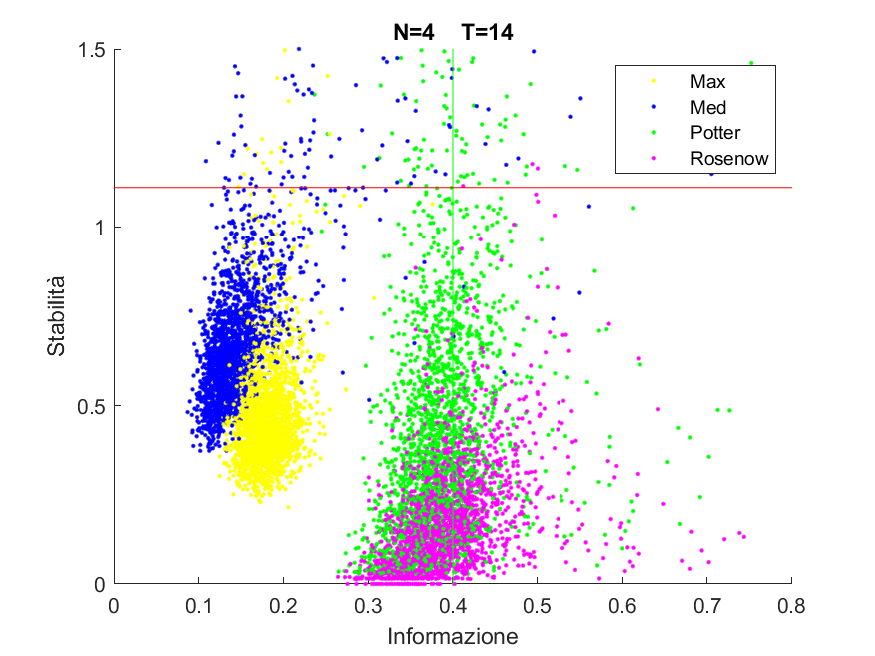
\includegraphics[width=\linewidth]{plot/pratici/Plot_n4_T14.png}
\end{column}
\begin{column}{0.33\linewidth}
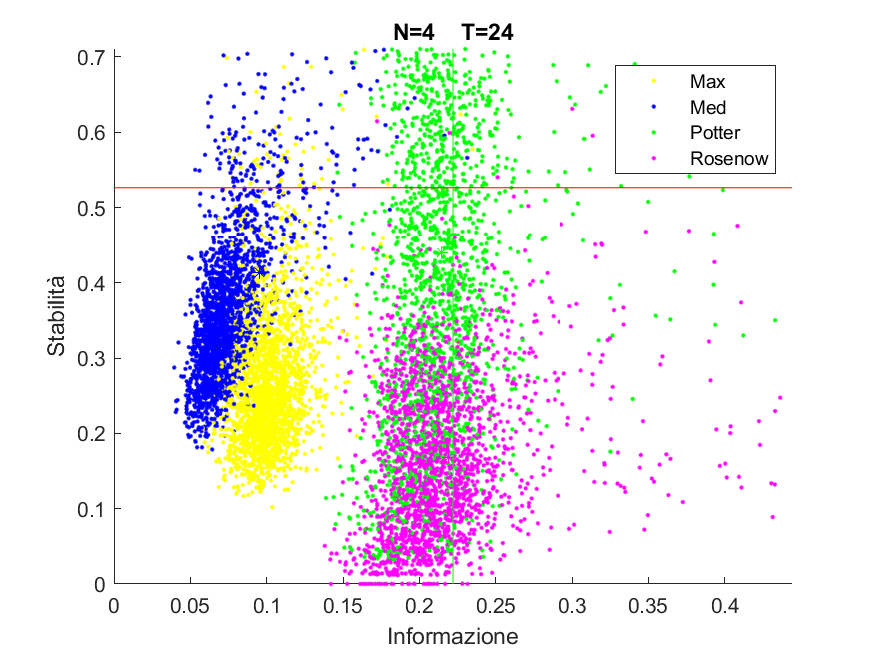
\includegraphics[width=\linewidth]{plot/pratici/Plot_n4_T24.png}
\end{column}
\end{columns}
\end{frame}

\begin{frame}{Applicazione - Test Pratici (n=10)}
\begin{columns}
\begin{column}{0.5\linewidth}
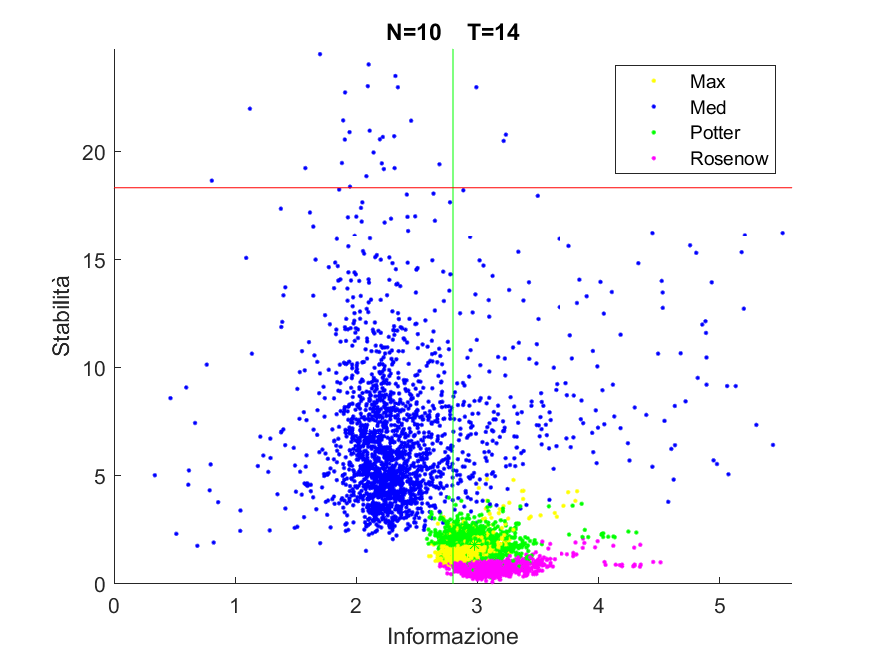
\includegraphics[width=\linewidth]{plot/pratici/Plot_n10_T14.png}
\end{column}
\begin{column}{0.5\linewidth}
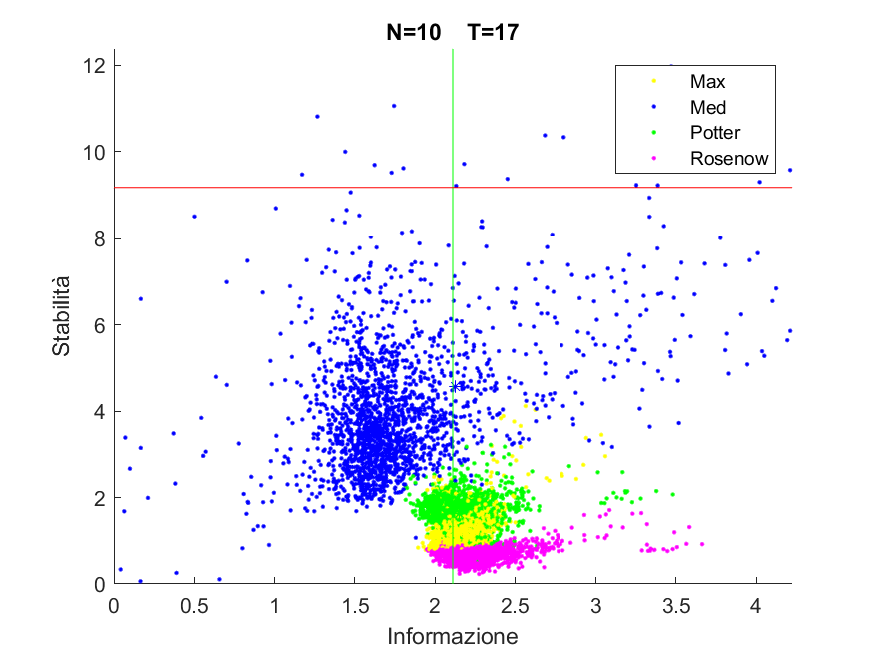
\includegraphics[width=\linewidth]{plot/pratici/Plot_n10_T17.png}
\end{column}
\end{columns}

\begin{columns}
\begin{column}{0.33\linewidth}
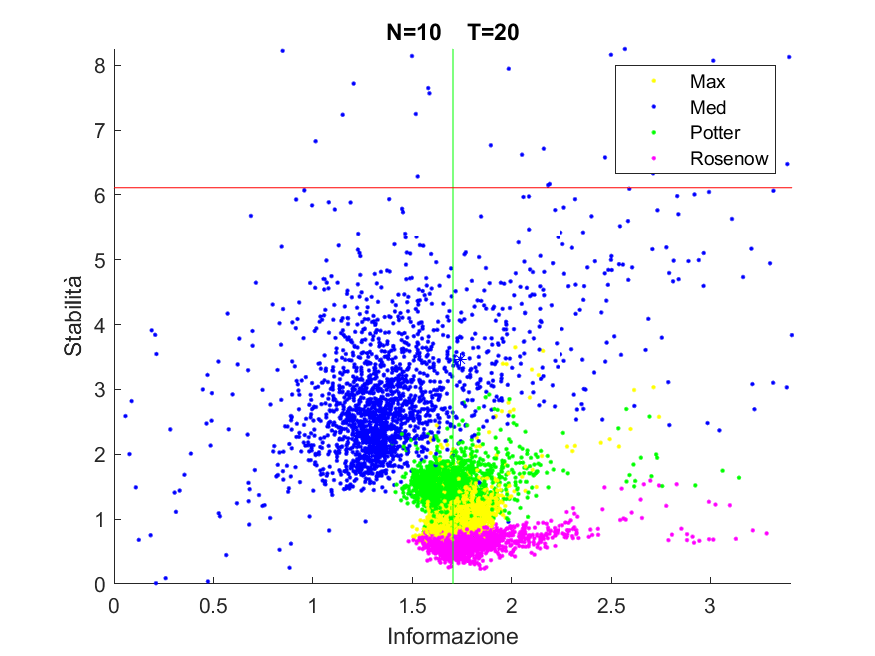
\includegraphics[width=\linewidth]{plot/pratici/Plot_n10_T20.png}
\end{column}
\begin{column}{0.33\linewidth}
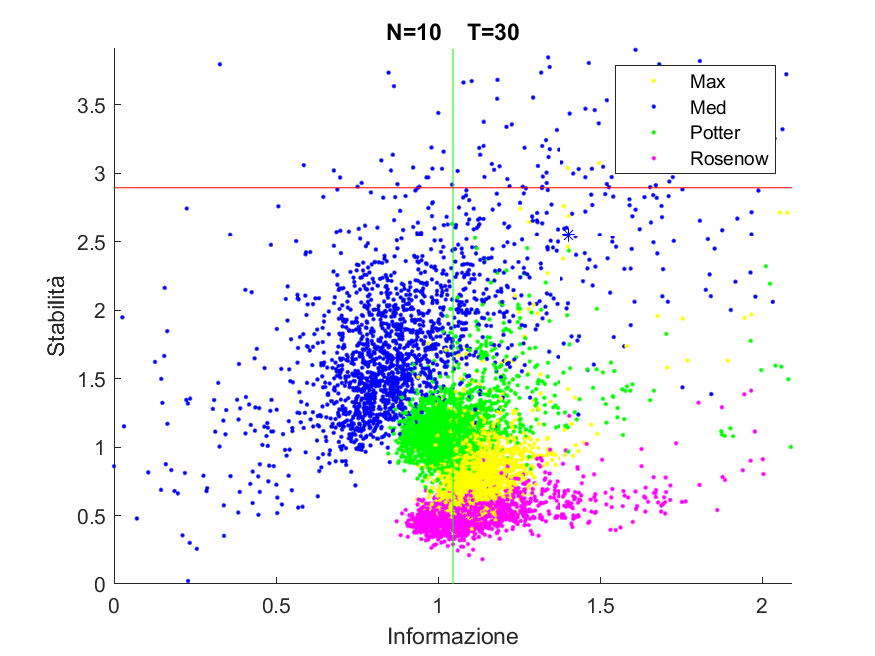
\includegraphics[width=\linewidth]{plot/pratici/Plot_n10_T30.png}
\end{column}
\begin{column}{0.33\linewidth}
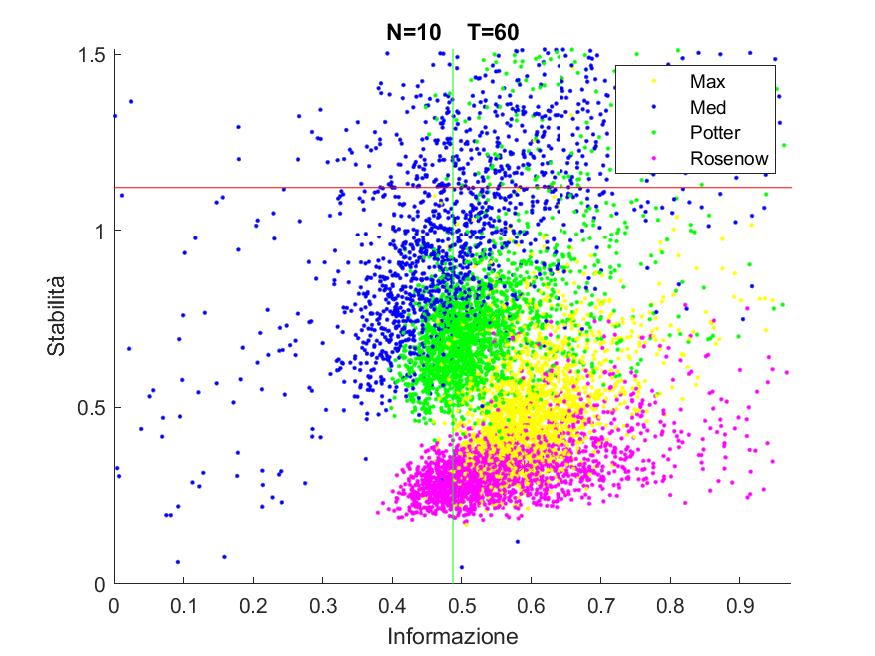
\includegraphics[width=\linewidth]{plot/pratici/Plot_n10_T60.png}
\end{column}
\end{columns}
\end{frame}


\begin{frame}{Proiettile di Markowitz}
Sia dato un mercato con vettore dei ritorni attesi $M$ e covarianza $\Sigma$.
\vspace{10pt}

\begin{block}{Definizione}
Un \textbf{portfolio} è un vettore $W\in \{[0,1]\}^n$ di pesi.\\
$W_i$ è la percentuale del capitale che investiamo nello stock $i$. $\left( \sum W_i = 1 \right) $
\end{block}
Il ritorno atteso è quindi $\mu=MW^T$ e la varianza è $\sigma^2=W\Sigma W^T$.\\
\vspace{20pt}

C'è un ordinamento parziale nell'insieme $\mathcal{W}$ dei portafogli.
\[
W_1\preceq W_2 \quad\Leftrightarrow\quad \mathbb{E}[W_1]\leq\mathbb{E}[W_2] \,\wedge\, \text{Var}(W_1)\geq\text{Var}(W_2)
\]
\vspace{-15pt}
\begin{block}{Definizione}
Un portfolio si dice \textbf{efficiente} se è un elemento massimale rispetto a $\preceq$
\end{block}
\end{frame}

\begin{frame}{Proiettile di Markowitz}
\begin{block}{Markowitz}
Dato $\mu\in\bbR^+$, il portfolio con ritorno atteso $\mu$ e varianza minima ha pesi:
\[
W=
\frac{
\det\left(
	\begin{array}{cc}
		\mu & M\Sigma^{-1}\mathbbm{1}^T\\
		1   & \mathbbm{1}\Sigma^{-1}\mathbbm{1}^T
	\end{array}
\right)M\Sigma^{-1}
+
\det\left(
	\begin{array}{cc}
		M\Sigma^{-1}M^T     &  \mu\\
		\mathbbm{1}\Sigma^{-1}M^T  & 1
	\end{array}
\right)\mathbbm{1}\Sigma^{-1}
}
{
\det\left(
	\begin{array}{cc}
		M\Sigma^{-1}M^T  &  M\Sigma^{-1}\mathbbm{1}^T\\
		\mathbbm{1}\Sigma^{-1}M^T  &  \mathbbm{1}\Sigma^{-1}\mathbbm{1}^T
	\end{array}
\right)
}
\]
\end{block}
\vspace{10pt}

\begin{columns}
\begin{column}{0.5 \textwidth}
Possiamo quindi tracciare la curva dei portafogli efficienti, il cosiddetto proiettile di Markowitz
\end{column}
\begin{column}{0.5 \textwidth}
\includegraphics[width=\linewidth]{mark.png}
\end{column}
\end{columns}
\end{frame}


\begin{frame}{Criterio di Kelly}
Supponiamo che a un giocatore venga data la possibilità di scommettere una fissata frazione $f$ del suo capitale (arbitrariamente divisibile) su lanci successivi di monete.\\
Ad ogni lancio con probabilità $p<\frac{1}{2}$ vince quanto ha scommesso, con probabilità $1-p$ perde.
\vspace{15pt}

Quale $f$ scegliere?
\begin{itemize}
\item $f=1$ massimizza il valore atteso
\item $f=0$ minimizza la varianza
\end{itemize}
\end{frame}

\begin{frame}{Criterio di Kelly}
Se $F_n$ è il capitale al passo $n$, definiamo il grow rate esponenziale come
\[
G:=\lim_{n\to\infty}\log
\left(\left(
\frac{F_n}{F_0}\right)^{\frac{1}{n}}\right)
\]
Se il giocatore dopo $n$ passi ha vinto W volte e perso L volte, $F_n=(1+f)^W(1-f)^LF_0$, e quindi
\[
G =
\lim_{n\to\infty}
\left(
	\frac{W}{n}\log(1+f)+
	\frac{L}{n}\log(1-f)
\right)
=
p\log(1+f) + (1-p) \log(1-f)
\]
\begin{block}{Il criterio di Kelly}
Se definiamo $f^*_{ottimale} := \arg\min \left\{\mathbb{E}[\log(return(f^*))] \,:0\leq f^*\leq1 \right\} $ \\
\vspace{5pt}
Per scommesse semplici con due possibili risultati vale:
\[ f^*= p-(1-p) \]
\end{block}
%Il criterio di Kelly si utilizza per determinare la percentuale $f^*$ ottimale del capitale da investire in una scommessa.
\end{frame}








\begin{frame}{Check Risultati}
\begin{columns}
\begin{column}{0.5\linewidth}
\includegraphics[width=\linewidth]{plot/teorici/FANCY/Plot_n4_T6_it100_simul1000.png}
\end{column}
\begin{column}{0.5\linewidth}
\includegraphics[width=\linewidth]{plot/teorici/FANCY/Plot_n4_T8_it100_simul1000.png}
\end{column}
\end{columns}
\begin{columns}
\begin{column}{0.33\linewidth}
\includegraphics[width=\linewidth]{plot/teorici/FANCY/Plot_n4_T11_it100_simul1000.png}
\end{column}
\begin{column}{0.33\linewidth}
\includegraphics[width=\linewidth]{plot/teorici/FANCY/Plot_n4_T14_it100_simul1000.png}
\end{column}
\begin{column}{0.33\linewidth}
\includegraphics[width=\linewidth]{plot/teorici/FANCY/Plot_n4_T24_it100_simul1000.png}
\end{column}
\end{columns}
\end{frame}

\begin{frame}{Check Risultati}
\begin{columns}
\begin{column}{0.5\linewidth}
\includegraphics[width=\linewidth]{plot/teorici/FANCY/Plot_n10_T14_it100_simul1000.png}
\end{column}
\begin{column}{0.5\linewidth}
\includegraphics[width=\linewidth]{plot/teorici/FANCY/Plot_n10_T17_it100_simul1000.png}
\end{column}
\end{columns}
\begin{columns}
\begin{column}{0.33\linewidth}
\includegraphics[width=\linewidth]{plot/teorici/FANCY/Plot_n10_T20_it100_simul1000.png}
\end{column}
\begin{column}{0.33\linewidth}
\includegraphics[width=\linewidth]{plot/teorici/FANCY/Plot_n10_T30_it100_simul1000.png}
\end{column}
\begin{column}{0.33\linewidth}
\includegraphics[width=\linewidth]{plot/teorici/FANCY/Plot_n10_T60_it100_simul1000.png}
\end{column}
\end{columns}
\end{frame}

\begin{frame}{Check Risultati}
\begin{columns}
\begin{column}{0.5\linewidth}
\includegraphics[width=\linewidth]{plot/teorici/angolo/Plot_n4_T6_it100_simul1000.png}
\end{column}
\begin{column}{0.5\linewidth}
\includegraphics[width=\linewidth]{plot/teorici/angolo/Plot_n4_T8_it100_simul1000.png}
\end{column}
\end{columns}
\begin{columns}
\begin{column}{0.33\linewidth}
\includegraphics[width=\linewidth]{plot/teorici/angolo/Plot_n4_T11_it100_simul1000.png}
\end{column}
\begin{column}{0.33\linewidth}
\includegraphics[width=\linewidth]{plot/teorici/angolo/Plot_n4_T14_it100_simul1000.png}
\end{column}
\begin{column}{0.33\linewidth}
\includegraphics[width=\linewidth]{plot/teorici/angolo/Plot_n4_T24_it100_simul1000.png}
\end{column}
\end{columns}
\end{frame}

\begin{frame}{Check Risultati}
\begin{columns}
\begin{column}{0.5\linewidth}
\includegraphics[width=\linewidth]{plot/teorici/angolo/Plot_n10_T14_it100_simul1000.png}
\end{column}
\begin{column}{0.5\linewidth}
\includegraphics[width=\linewidth]{plot/teorici/angolo/Plot_n10_T17_it100_simul1000.png}
\end{column}
\end{columns}
\begin{columns}
\begin{column}{0.33\linewidth}
\includegraphics[width=\linewidth]{plot/teorici/angolo/Plot_n10_T20_it100_simul1000.png}
\end{column}
\begin{column}{0.33\linewidth}
\includegraphics[width=\linewidth]{plot/teorici/angolo/Plot_n10_T30_it100_simul1000.png}
\end{column}
\begin{column}{0.33\linewidth}
\includegraphics[width=\linewidth]{plot/teorici/angolo/Plot_n10_T60_it100_simul1000.png}
\end{column}
\end{columns}
\end{frame}

\end{document}
